\documentclass[9pt,conference]{IEEEtran}
\usepackage{listings}
\usepackage{graphicx}
\usepackage[colorlinks,allcolors=blue]{hyperref}
\graphicspath{{./images/}}




\begin{document}


    \title{Quality assurance of digital twins -- An experience report in the automotive industry}
    \author{
        \IEEEauthorblockN{
            Georg Hackenberg
        }
        \IEEEauthorblockA{
            School of Engineering\\
            University of Applied Sciences Upper Austria\\
            4600 Wels, Upper Austria, Austria\\
            \href{mailto:georg.hackenberg@fh-wels.at}{georg.hackenberg@fh-wels.at}
        }
        \and
        \IEEEauthorblockN{
            Alican Tüzün
        }
        \IEEEauthorblockA{
            School of Engineering\\
            University of Applied Sciences Upper Austria\\
            4600 Wels, Upper Austria, Austria\\
            \href{mailto:alican.tuezuen@fh-wels.at}{alican.tuezuen@fh-wels.at}
        }
    }
    \maketitle

    \begin{abstract}
        Digital twins are becoming more and more important for the efficient and effective development and operation of cyber-physical systems.
        However, digital twins are only useful if they reflect the real-world system accurately enough, i.e.\ their quality is high enough.
        This claim entails the question, of what the term quality in the context of digital twins means and how it can be measured.
        In this article, we present our experience with the quality assurance of a digital twin for an assembly line in the automotive industry.
        We explain our preliminary definition of digital twin quality, which we derive from classical quality models for general software systems.
        Furthermore, we describe quality issues, which we were able to detect in a digital twin of an assembly line in the automotive industry.
        Finally, we conclude how to leverage our experience in different contexts and how to generalize the underlying approaches.
    \end{abstract}

    \section{Introduction}\label{section:introduction}

    Cyber-physical system (CPS), is a conceptual architecture/approach which aims to conjoin the physical and virtual space tightly. 
    The CPS aims to integrate communication and computing capabilities to physical entities to monitor, coordinate and control the physical space (where the physical assets exist) from the virtual space (where the virtual models exist) while achieving seamless, real-time connection between the spaces.
    The Digital twin approach, on the other hand, is a pragmatic solution, which is the execution of the CPS idea.~\cite{TAOCHAPTER1}
    
    The first occurrence of the "Digital Twin" term was introduced by Dr.~Michael Grieves in 2003 at the University of Michigan while giving the Product Lifecycle Management (PLM) course.~\cite{DTGRIEVES}
    His introduction to the term was rather raw but still introduced a pragmatic solution to gather more data from the physical entities, to achieve the "Lean" idea.
    
    His approach has three dimensions, along with a physical entity, a virtual entity and a connection between these entities which constructed the main frame for today's evaluating digital twins.~\cite{DTGRIEVES}

    A physical entity exists only in the physical space with real functionalities and performance. It is responsible to accomplish certain tasks within the physical space, to give certain outputs.
    Different levels of abstraction can be usable for a physical entity such as an electric motor in the 1/10 of an RC Car, bearings in a certain machine, solar panels above some construction, human or an entire world can be counted as an example of a physical entity.

    A virtual entity exists only in the virtual space, which should imitate the physical entity with high-fidelity models. If we consider the virtual entity as a function;

    \begin{equation}\label{Formulated Entity Equation}
        VE = (G_v, P_v, B_v, R_v)
    \end{equation}
    where:
    
    $G_v$ represents the geometry model, $P_v$ represents the physical model, $B_v$ represents  the behavior model, and $R_v$ represents the rule model~\cite{DTGRIEVES}.
    
    The last dimension is the connection between physical space and virtual space. Physical space created real-time data, and through the connection, these data will be received by the virtual space 
    and updates the states of the models. Virtual space sends the needed information to the physical space. 

    There is also another, an up-to-date approach that adds two more dimensions(Data and Services), to the traditional digital twin model which is described above.~\cite{DTGRIEVES}

    \begin{equation}
        M_{dt} = (PE,VE,Ss,DD,CN)
    \end{equation}

    \begin{description}
        \item[PE] Represents DT Physical Entity
        \item[VE] Represents DT Virtual Entity
        \item[Ss] Represents DT Services
        \item[DD] Represents DT Data
        \item[CN] Represents DT Connections
    \end{description}
    If we consider the dimensions we above discussed as vertical dimensions, if we divide our digital twin horizontally into three different layers, the explanation of the digital twin systems becomes much clearer.
    \begin{itemize}
        \item Unit DT which only has one PE in the physical space
        \item System DT  is an assembly of PE's in the physical space
        \item System of Systems DT  is an assembly of systems in the physical space
    \end{itemize} 

    Of course, there are other explanations, approaches, and architectures to digital twins, but like every other digital transformation approach, the main goal is to get into the lean state,
    which is an optimal approach to our problem. 
    
    Also should be noted that the digital twin approach was introduced within the PLM course. PLM is nothing but an improvement to the lean manufacturing philosophy, which aims to eliminate waste(Time, energy, Material) not only during the
    manufacturing process but also during the lifecycle of the product.~\cite{grieves2006PLM} 
    It's an approach to achieve the lean state, which overlaps with the idea of digital twins, which both aim to gather more information about the product, starting from the design phase to the disposal of the product.
    

    Achieving a full-scale cyber-physical system is not only a goal for the digital twin but also an essential challenge. The following are some examples of the challenges which is occurring during the development of a digital twin:
    \begin{itemize}
        \item High fidelity modeling and simulation
        \item Real-Time communication between the components of digital twin 
        \item Flexible data architecture
        \item Developing standards and protocols for the use of digital twins so that they can be used consistently across different industries and applications.
        \item Cost and Cost Management
        \item Cyber Security
        \item Quality Assurance of the digital twin
        \item Information inefficiency regarding the theme Digital Twins
        \item \dots{}
    \end{itemize}
    
    %TODO: How we are writing this?
    \subsection{Research objectives}
    
    Find an approach to assess the quality of Digital twins

    \subsection{Research questions}~\label{section: Research Questions}

    What is the quality of digital twins? 
    What is good quality?
    What is bad quality? 
    What is the impact of good quality? 
    What is the impact of bad quality? W
    What are typical quality issues? 
    How to assess quality?

    \subsection{Scientific contributions}

    Literature review (see Section~\ref{section: literature}), case study (see Section~\ref{section: Research Questions})...
    
    \section{Literature review}~\label{section: literature}
    Literature analysis was executed, to analyze current DT literature within the concept of digital twin quality. The analysis especially focused on 
    how the digital twin quality is mentioned and assessed within the academic dissertations.

    Methodology (see Section~\ref{section:liteature_methodology}), result (see Section~\ref{section:liteature_result}), and summary (See Section~\ref{section:liteature_summary})...
    \subsection{Methodology}~\label{section:liteature_methodology}
    Google Scholar (GS), Scopus (SCP) and Research Rabbit (RR) tools are used to fulfill our requirements for the literature review. 
    Since there is a great number of digital twin publications in academics, 
    narrowing the research is necessary, so the following algorithm which can be seen in Figure \ref{fig:literaturesearchalgorithm} with several levels of filtering will be applied.
    
    First filtering will be done with the following criteria:
    \begin{itemize}
        \item Dissertations should be written in English and published in a journal/conference.
        \item Paper is not older than 2018
        \item Search term should be exactly searched.
    \end{itemize}

   
    Filtering query calls for the GS and SCP are the following:
    \begin{itemize}
        \item Google Scholar = "search term"
        \item Scopus = ALL ( "digital twin quality" ) AND PUBYEAR > 2018 AND PUBYEAR < 2023 AND ( LIMIT-TO ( LANGUAGE , "English" )) 
    \end{itemize} 

    Also want to note that, in the GS, there isn't a function that filters the dates, instead the user should click the Since 2018 option to filter the dates.


    Second filtering will be done to eliminate the duplications, which can occur when GS and SCP give the same result.
    \begin{itemize}
        \item Remove Duplications
        \item Remove the dissertations which are not English manually
    \end{itemize}  
    
    Even though we already filtered the language, still some dissertations results will appear because of the auto translation which they put on the website.
    So second time should be filtered manually.

    After the second filtration, the third filtering which is a manual investigation should occur with the following filtering criteria:
    \begin{itemize}
        \item Proper literature review should be present in the selected paper
        \item Abstract and conclusion should be relevant to the search term
    \end{itemize}
    
    \begin{figure}
        \centering
        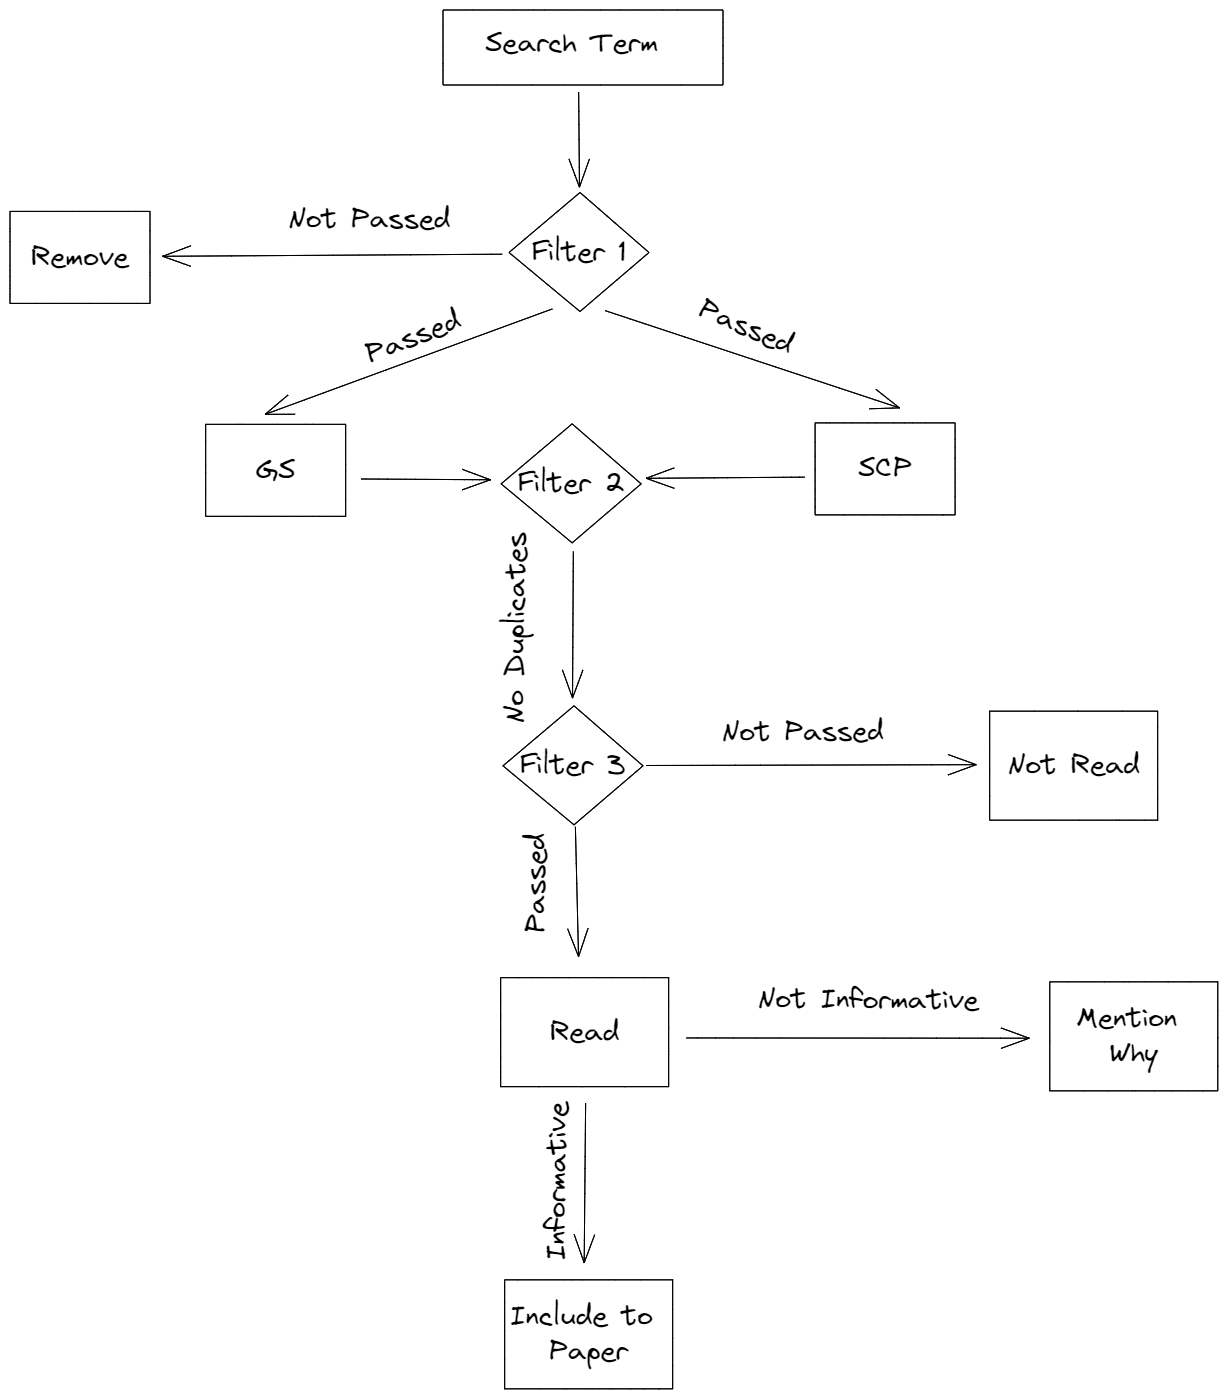
\includegraphics[width =0.45\textwidth]{LRMethod.png}
        \caption{Literature Search Algorithm}
        \label{fig:literaturesearchalgorithm}
    \end{figure} 
    \begin{figure}
        \centering
        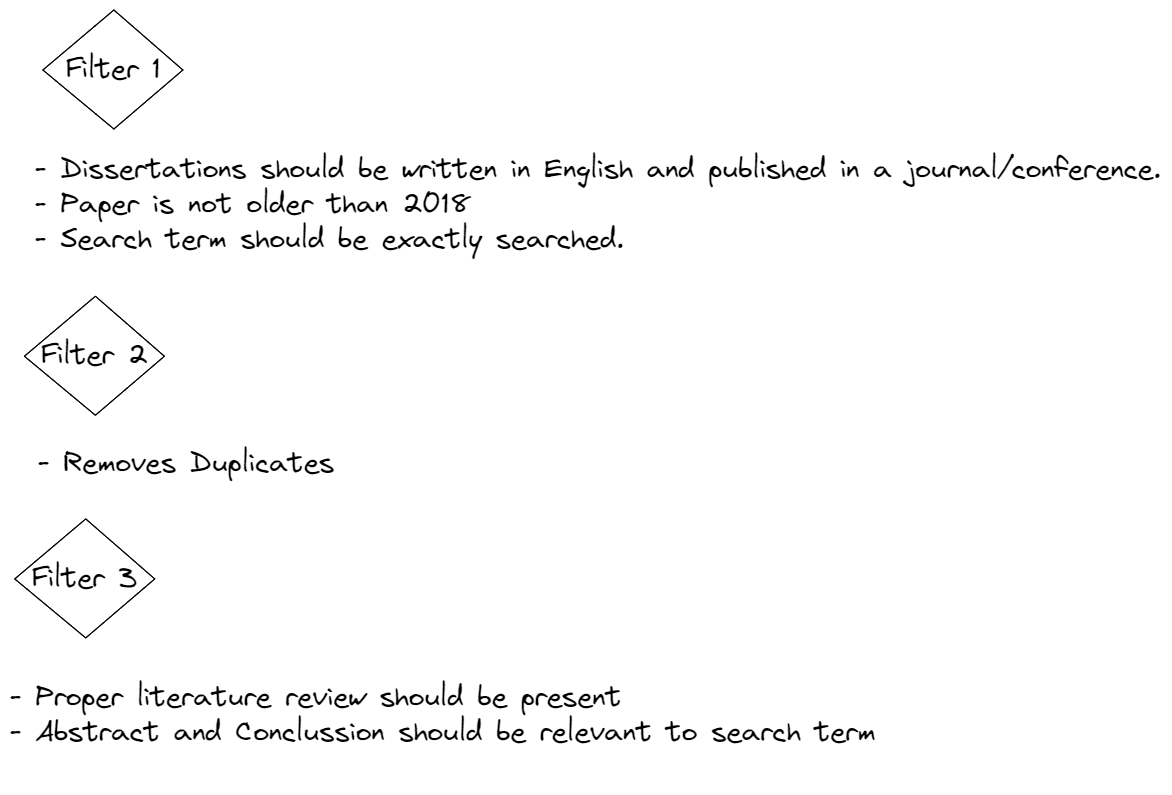
\includegraphics[width =0.45\textwidth]{LRMethodLegacy.png}
        \caption{Literature Search Algorithm Legend}
        \label{fig:literaturesearchalgorithmlegend}
    \end{figure}

    

    %TODO: ADD THE METHOD HERE

    
    \subsection{Result}~\label{section:liteature_result}
    The following results were achieved by selecting several  search terms, which is 
    \subsubsection*{Digital Twin Quality}\label{subsection:Digital Twin Quality}
    
    First filtering is done for the search term "digital twin quality", meanwhile GS gave 41 different results, and SCP gave only 3 results.
    After the second filtering process, 3 duplications and 31 different results were found. 10 dissertations were not in English.
    After the third filtering process, 9 dissertations passed and the rest is rejected.

    \subsubsection*{Digital Twin Testing}\label{subsection:Digital Twin Quality}
    %What is the existing literature?

    \subsection{Summary}~\label{section:liteature_summary}

    What do we learn from existing literature?
    (Existing literature does at most partially solve our problem!)

    \section{Case study (FELICE)}~\label{section:case}

    TODO (Explain the limitations of the FELICE digital twin! It is not a complete digital twin according to literature! It includes this, it is missing this.)

    \subsection{Methodology}~\label{section:case_methodology}

    TODO

    \subsection{Result}~\label{section:case_result}

    TODO

    \subsection{Summary}~\label{section:case_summary}

    TODO

    \section{Conclusion}~\label{section:conclusion}
    TODO

    \section*{Acknowledgements}
    TODO

    \bibliography{main}
    \bibliographystyle{plain}

\end{document}